
%(BEGIN_QUESTION)
% Copyright 2011, Tony R. Kuphaldt, released under the Creative Commons Attribution License (v 1.0)
% This means you may do almost anything with this work of mine, so long as you give me proper credit

Explain where and how TIR-38 and DIR-38 get their data to display to the operators, based on the information in this P\&ID for a waste gas incinerator:

$$\includegraphics[width=15.5cm]{i0004rx01.eps}$$

\vfil 

\underbar{file i03238}
\eject
%(END_QUESTION)





%(BEGIN_ANSWER)

This is a graded question -- no answers or hints given!
 
%(END_ANSWER)





%(BEGIN_NOTES)

Flow transmitter FT-38 is a {\it coriolis} flow transmitter transmitter, sensing mass flow rate, density, and tube temperature.  FY-38c is a HART multivariable converter, polling temperature and density data from FT-38 and repeating it in analog form to indicators TIR-38 and DIR-38.

%INDEX% Fieldbus, HART: multivariable instrument (realistic P&ID shown)
%INDEX% Process: incinerator (realistic P&ID shown)

%(END_NOTES)


